%%%%%%%%%%%%%%%%%%%%%%%%%%%%%%%%%%%%%%%%%
% fphw Assignment
% LaTeX Template
% Version 1.0 (27/04/2019)
%
% This template originates from:
% https://www.LaTeXTemplates.com
%
% Authors:
% Class by Felipe Portales-Oliva (f.portales.oliva@gmail.com) with template 
% content and modifications by Vel (vel@LaTeXTemplates.com)
%
% Template (this file) License:
% CC BY-NC-SA 3.0 (http://creativecommons.org/licenses/by-nc-sa/3.0/)
%
%%%%%%%%%%%%%%%%%%%%%%%%%%%%%%%%%%%%%%%%%

%----------------------------------------------------------------------------------------
%	PACKAGES AND OTHER DOCUMENT CONFIGURATIONS
%----------------------------------------------------------------------------------------

\documentclass[
	12pt, % Default font size, values between 10pt-12pt are allowed
	%letterpaper, % Uncomment for US letter paper size
	%spanish, % Uncomment for Spanish
]{fphw}

% Template-specific packages
\usepackage[utf8]{inputenc} % Required for inputting international characters
\usepackage[T1]{fontenc} % Output font encoding for international characters
\usepackage{multicol, latexsym, amsmath, amssymb}
\usepackage{blindtext}
\usepackage{subcaption}
\usepackage{caption}
\usepackage{wrapfig}
\usepackage{tabu}
\usepackage{floatflt}
\usepackage{graphicx} % Required for including images

\usepackage{booktabs} % Required for better horizontal rules in tables

\usepackage{listings} % Required for insertion of code

\usepackage{enumerate} % To modify the enumerate environment


%----------------------------------------------------------------------------------------
%	ASSIGNMENT INFORMATION
%----------------------------------------------------------------------------------------

\title{Assignment 1} % Assignment title

\author{Giuliano  1234567, Gabriele Giannotta 1909375, Mario Dhimitri 1234567 } % Student name

\date{October 30th, 2020} % Due date

\institute{Sapienza Università di Roma \\ Data Science} % Institute 

\class{Advanced Machine Learning} % Course or class name

\professor{Fabio Galasso} % Professor 

%----------------------------------------------------------------------------------------

\begin{document}

\maketitle % Output the assignment title, created automatically using the information in the custom commands above

%----------------------------------------------------------------------------------------
%	ASSIGNMENT CONTENT
%----------------------------------------------------------------------------------------

\section*{Report 1 - Image Filtering}

Write here your report


\newpage
\section*{Report 2 - Object Identification}


In order to find the best combination to get a better result, we computed the recognition rate for all the possible combinations of the three type of distance (intersect, l2, chi2) with respect to the histogram functions (rgb, rg, dxdy), considering 6 different number of bins (5,10,15,20,30,50) for each combination. After that, the obtained results were inserted in a dataframe and analyzed with Pandas tools. \\
From the 54 combinations analyzed, the following results were obtained:\\ \\


\begin{figure*}[h!]
    \centering
    \begin{subfigure}[t]{0.5\textwidth}
        \centering
        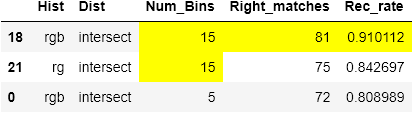
\includegraphics[height=0.9in]{img/best_combination.png}
         \caption{Best Combination}
    \end{subfigure}%
    ~ 
    \begin{subfigure}[t]{0.5\textwidth}
        \centering
        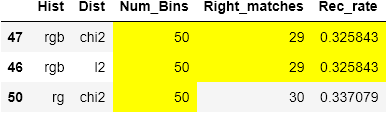
\includegraphics[height=0.9in]{img/worst_combination.png}
         \caption{Worst Combination}
	\end{subfigure}

\end{figure*}


The best combination found is: \{Histogram: rgb; Distance: Intersect; Number of Bins: 15\}, with a number of matches of 81 out of 89 ( Recognition Rate = 0.91 ).\\ 

The worst combination found is: \{Histogram: rgb; Distance: chi2; Number of Bins: 50\}, with a number of matches of 29 out of 89 ( Recognition Rate = 0.32 ).\\

Finally, looking specifically at the distance type, we noticed that on average the intersect distance was the best for each type of histogram.
The average is calculated taking into account the six test cases \(num_bins = 5, 10, 15, 20, 30, 50\).

\begin{figure*}[h!]
    \centering
    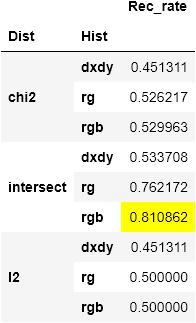
\includegraphics[height=2.8in]{img/best_dist.png}
     \caption{Best Distance}
\end{figure*}



\newpage
\section*{Report 3 - Performance Evaluation}

Write here your report






%------------------------------------------------
\end{document}
